\chapter{Cellular Occupancy and Habitat Spaces}

\section{Occupancy as a Rule}

Chapter 15 grew a structure by adding one particle at a time. A second way of forming structure without a plan keeps the lattice fixed and decides, for every site, whether it is occupied. The simplest such rule treats the sites independently: each site is occupied with probability $p$, by a draw that does not depend on any other site. The result is a random field with a single parameter, and it is the starting point for two questions that matter when the field is meant to be a space that someone can move through. The first is whether the occupied sites, or the empty ones, form a connected region that crosses the whole grid. The second is what a local rule applied repeatedly to the field does to its connectivity. This chapter measures both on a square grid and then places the result in Blender as a habitat floor plan, with the same attention to provenance as before.

Four things have to be stated for the rule to be complete: the grid size $n$, the occupation probability $p$, the notion of adjacency, and the generator with its seed. Adjacency matters because it changes the answer. Two sites are \emph{four-adjacent} if they share an edge and \emph{eight-adjacent} if they share an edge or a corner. A region of occupied sites is a set connected through the chosen adjacency, and a region that touches both the top row and the bottom row is said to span. All counts below use four-adjacency for connection of a region, and the smoothing rule of Section 16.4 uses the eight sites around a cell.

The code is in \texttt{occupancy.py}. The generator is NumPy's \texttt{default\_rng} seeded by an integer, regions are labelled with SciPy's \texttt{ndimage.label}, and a grid built twice from seed $7$ at $n=64$, $p=0.45$ was identical site for site, while seed $8$ differed from it at $2042$ of $4096$ sites. The occupied fraction of the seed-$7$ grid was $0.455$ against a nominal $0.45$, a difference that is ordinary sampling variation, since the standard deviation of the fraction over $4096$ independent sites is $0.008$.

\section{When Occupied Sites Span}

Consider the probability that a random grid of side $n$ has a four-connected occupied region touching both the top and the bottom row. For small $p$ the occupied sites are isolated specks and the probability is near zero, and for $p$ near one it is near one. The interesting question is how sharp the change is and where it sits. The probability was estimated from $400$ seeds at each of seven values of $p$ and four grid sizes.

\begin{center}
\begin{tabular}{rrrrrrrr}
\toprule
$n$ & $p=0.50$ & $0.55$ & $0.58$ & $0.5927$ & $0.61$ & $0.65$ & $0.70$\\
\midrule
32  & 0.013 & 0.125 & 0.335 & 0.440 & 0.635 & 0.915 & 0.990\\
64  & 0.000 & 0.065 & 0.325 & 0.547 & 0.807 & 0.985 & 1.000\\
128 & 0.000 & 0.003 & 0.195 & 0.487 & 0.912 & 1.000 & 1.000\\
256 & 0.000 & 0.000 & 0.072 & 0.515 & 0.983 & 1.000 & 1.000\\
\bottomrule
\end{tabular}
\end{center}

Each entry has a binomial standard error of at most $0.025$. The table shows the change sharpening with $n$: at $p=0.55$ the spanning probability falls from $0.125$ to below $0.005$ as $n$ grows from $32$ to $256$, and at $p=0.61$ it rises from $0.635$ to $0.983$. Curves for different $n$ cross close to $p=0.59$, where the probability is near one half at every size. A sharper measurement of the location is the value of $p$ at which the spanning probability equals one half, found by bisection with $400$ seeds at each step. It was $0.5979$, $0.5907$, $0.5933$ and $0.5925$ for $n=32$, $64$, $128$, $256$. The scatter among the last three, about $0.003$, is of the size expected from $400$ seeds, so the data support a threshold near $0.59$ and no drift in it beyond that scatter. The value usually quoted for site percolation on the square lattice, $0.5927$, is recalled from reading and was not derived here, and these numbers agree with it to the precision measured.

Two points follow for design. A spanning region is not a gradual achievement: a grid with $p=0.55$ of its sites open, which is more than half, is very unlikely to be crossable by four-adjacent steps, and the same grid at $p=0.65$ almost certainly is. And the answer depends on the adjacency, so a rule for walking must be fixed before a field is judged crossable.

\section{Occupancy as a Floor Plan}

A random field is not a plan, but it is the raw material of one common approach to generating caves and ruins, so it is worth stating what the approach would require. Take occupied to mean wall. The open space is the complement, and a visitor can cross it only if the open sites span, so the open-site probability $1-p$ must exceed the threshold, and $p$ must be below about $0.41$. For walls at $p=0.45$ the open fraction is $0.55$, and the table says that open space spanning the grid is rare. A direct count on $200$ grids of $64\times 64$ at $p=0.45$ gave a mean of $200.7$ separate open regions, the largest holding on average $20.2\%$ of the open sites. This is not a space but dust.

\section{A Local Rule Repeated}

The standard remedy is a smoothing rule applied to every cell at once. A cell becomes wall at the next step if at least five of the nine cells in its neighbourhood, itself included, are wall, and becomes open otherwise; cells outside the grid count as wall. The rule is synchronous, so the new grid is computed entirely from the old one. It is the majority rule on an odd number of cells, so it has no ties. Repeated, it either reaches a grid that no longer changes or it does not, and both outcomes occurred.

\begin{center}
\begin{tabular}{rrrrrr}
\toprule
$p$ & Steps & Fixed\,\% & Regions & Largest & Open\\
\midrule
0.40 & $18.4\pm 5.3$ & 100\% & 1.2 & 0.999 & 0.830\\
0.45 & $19.8\pm 7.7$ & 100\% & 2.0 & 0.985 & 0.668\\
0.50 & $22.0\pm13.6$ & 98\%  & 7.3 & 0.665 & 0.444\\
0.55 & $20.9\pm 7.8$ & 100\% & 14.4 & 0.293 & 0.222\\
0.60 & $18.2\pm 5.0$ & 100\% & 11.1 & 0.250 & 0.081\\
\bottomrule
\end{tabular}
\end{center}

The columns give the wall fraction $p$, the steps to a fixed point (mean and standard deviation across seeds), the percentage of grids that reached one within $100$ steps, the number of open regions, the share of open sites in the largest region, and the open fraction after smoothing. The figures are means over $200$ seeds on a $64\times64$ grid, with the region columns taken after smoothing. The rule turns the dust of $p=0.45$ into a nearly single space: $200.7$ open regions before, $2.0$ after, with the largest holding $98.5\%$ of the open sites. The open fraction rises from $0.55$ to $0.668$, which is the rule amplifying the majority, and not a change in the nominal parameter. The same rule at $p=0.55$ goes the other way and closes the field, leaving $14.4$ regions of which the largest holds under a third. The behaviour near $p=0.5$ is a separation between two regimes that the rule creates, a result of the rule and not of the percolation threshold, since smoothing at $p=0.45$ opens a space at an open fraction, $0.55$, below the threshold $0.5927$ that a random field would need.

Five of the $200$ grids at $p=0.5$ did not reach a fixed point in $100$ steps. Examination of those five showed that each had settled into a cycle of period two, four cells flipping on every step. This is a known property of synchronous rules and it is why the statement ``iterate until nothing changes'' is not a safe definition of the procedure: a rule that is run for a fixed number of steps, or that is checked for cycles, always terminates. A grid is declared a fixed point when one step returns it unchanged, so the fixed points reported are fixed by construction.

\section{The Grid in Blender}

Each wall cell becomes an object that shares one cube mesh, in the manner of Chapters 5 and 15, positioned at its integer coordinates and carrying as a custom property the number of wall cells among its eight neighbours. One material reads the property with an Attribute node and maps it from $0$ to $8$ through a two-colour ramp, so edges of walls, which have few wall neighbours, appear in warm colour and wall interiors in dark. The script is \texttt{occupancy\_blender.py}. The random grid and the smoothed grid of seed $3$ at $64\times 64$, $p=0.45$ were built side by side: $1845$ and $1476$ wall objects, one mesh with $3321$ users, and one material. Reading the cell positions back from the scene reproduced both grids exactly, the open regions counted from the scene were $201$ before and $2$ after, with largest-region fractions $0.204$ and $0.994$, regeneration of the smoothed grid from the seed and probability stored on its collection reproduced the scene, the fixed point was reached in $27$ steps, and one further application of the rule left the scene unchanged. Provenance in this chapter has an additional element that Chapter 15 did not need: the rule itself, which is stored as a string on the collection and which would have to match the code that regenerates the grid.

\begin{figure}[ht]
\centering
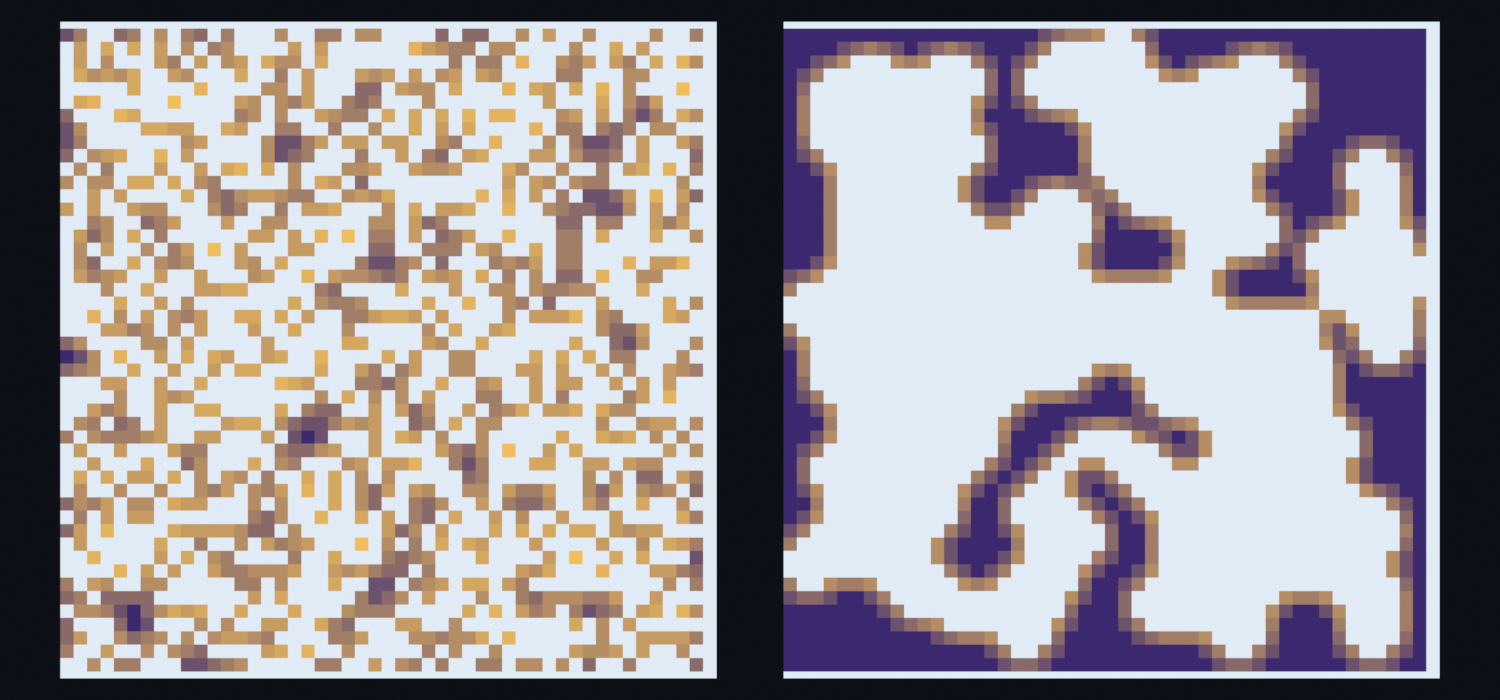
\includegraphics[width=\textwidth]{figs/fig16_caves.png}
\caption{A $48\times48$ random field of walls at $p=0.45$ (left) and the same field after the smoothing rule reached its fixed point (right), seed $3$, viewed from above in Blender. One material colours each wall cube by the number of wall cells among its eight neighbours, warm for few and dark for many. The open region on the right is connected; the field on the left has $133$ open regions and on the right it has $2$.}
\end{figure}

\section{What These Experiments Do Not Show}

All results are for square grids of at most $256\times256$ with four-adjacency for regions, at most $400$ seeds for the spanning estimates and $200$ for the smoothing statistics. The threshold values come from bisection with $400$ seeds per step and are good to about $0.003$; no finite-size scaling analysis was done, so nothing here establishes how the crossing probability depends on $n$ beyond what the table shows. The smoothing rule uses a single threshold of five of nine and a single boundary convention, and neither was varied, so the transition between open and closed outcomes near $p=0.5$ was not located more finely than the five values of the table. The period-two cycles were seen in five grids and were identified by inspection of those grids only. The comparison with the literature threshold is from recollection. Finally, a connected open region is not necessarily a good habitat: nothing was measured about corridor width, dead ends, or sight lines, and Chapter 9 showed that such properties can decide what a visitor can perceive. The experiment shows what the rule does to connectivity, with stated precision.

\begin{exercise}[16.1: Eight-adjacent regions]
Repeat the spanning estimate with eight-adjacency for the occupied region, find the half-probability value of $p$ for $n=128$, and compare it with $1-0.5927$. State why a relationship between the two numbers is to be expected, and test it.
\end{exercise}

\begin{exercise}[16.2: Move the rule]
Change the wall threshold from five of nine to four of nine and to six of nine, and for $p=0.45$ report the open fraction, the number of open regions, and the fraction of grids that cycle. State which of the three rules gives a usable space most often.
\end{exercise}

\begin{exercise}[16.3: Break the cycles]
Replace the synchronous update by one that updates the cells in a fixed scan order. Measure whether period-two cycles still occur, and describe what the change does to the dependence of the result on the seed and on the scan order.
\end{exercise}

\begin{exercise}[16.4: Walk it]
In Blender, place a unit-width walker at an open cell of the smoothed grid and find the shortest four-adjacent route to the farthest open cell. Report its length, compare it with the Manhattan distance between the endpoints, and explain what the ratio says about the corridors.
\end{exercise}
